\begin{frame}{Fine-Tuning Hyperparameters}
  \centering
  \renewcommand{\arraystretch}{1.2}
  \small
  \begin{tabular}{ll}
    \toprule
    \textbf{Parameter} & \textbf{Value} \\
    \midrule
    Base model            & Qwen2.5-14B-Instruct \\
    Quantization          & NF4 + double quantization \\
    LoRA rank / $\alpha$  & 64 / 128 \\
    Target layers         & All 48 layers \\
    Target modules        & q/k/v/o\_proj, gate/up/down\_proj \\
    Trainable parameters  & $\sim$275M (1.9\%) \\
    \midrule
    Training samples      & 2,625 unique (3,329 raw $-$ 704 deduped) \\
    & (2,074 Observer + 551 Operator) \\
    Teacher model         & GPT-5-mini (distilled traces) \\
    Epochs                & 3 \\
    Effective batch size  & 16 (micro=1, grad\_accum=16) \\
    Max sequence length   & 8,192 tokens \\
    Learning rate         & $1\times10^{-4}$ \\
    LR schedule           & Cosine with 5\% warmup \\
    Hardware              & 1$\times$ NVIDIA A40 (46 GB) \\
    Training cost         & $\approx$\$20 (cloud GPU) \\
    \bottomrule
  \end{tabular}
\end{frame}

\begin{frame}{Training Loss Curve (WandB)}
  \centering
  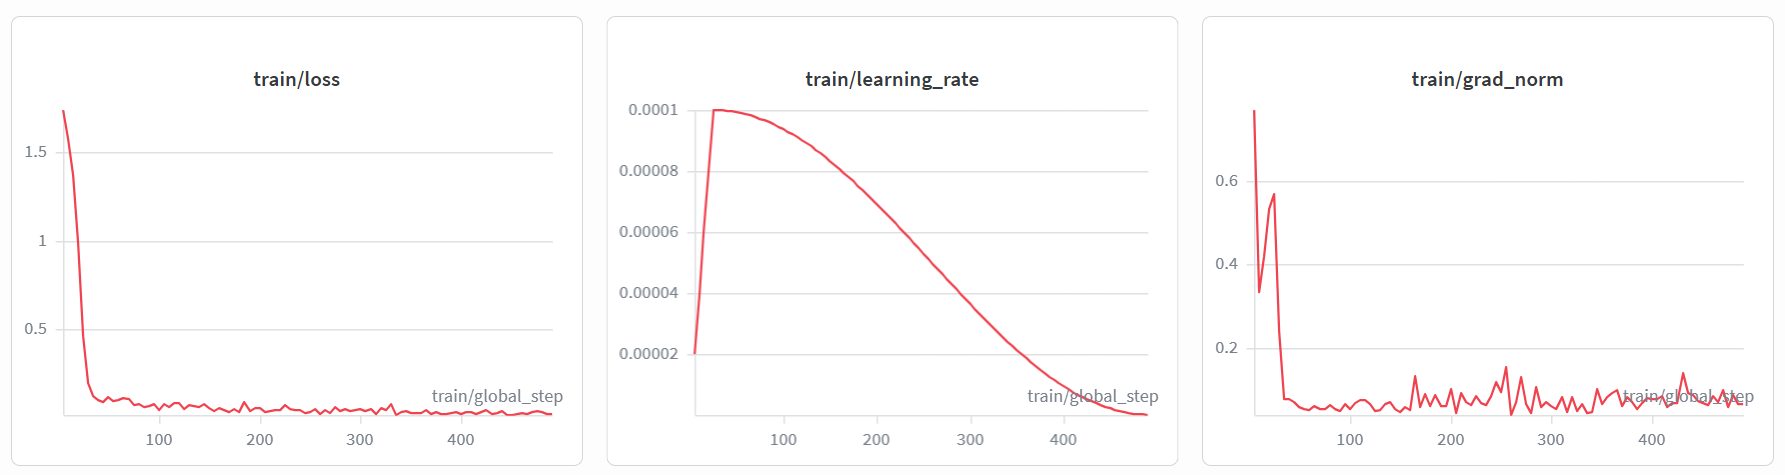
\includegraphics[width=0.9\textwidth]{../report/images/train_wandb.png}
  \captionof{figure}{Training loss over 3 epochs on 2,625 distilled samples. Cosine LR schedule with 5\% warmup; loss on assistant tokens only.}
\end{frame}

\begin{frame}{Benchmark Scenario Distribution}
  \centering
  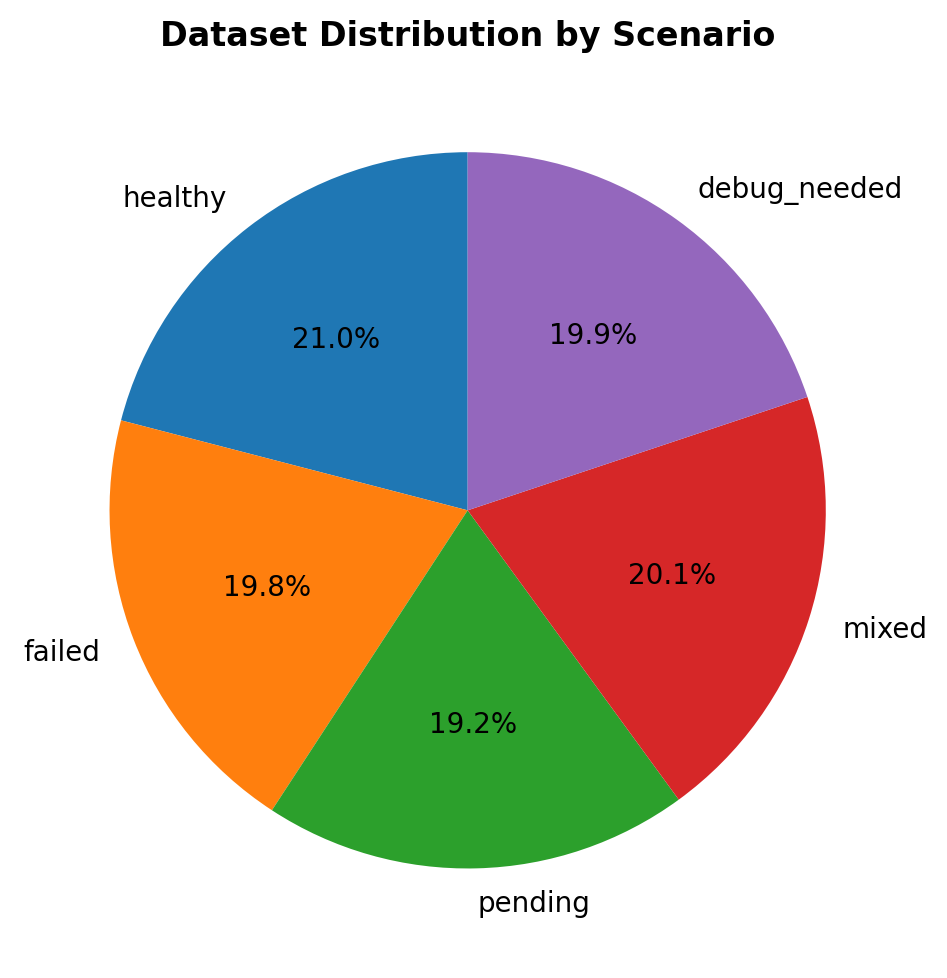
\includegraphics[width=0.7\textwidth]{../report/images/evaluation/scenario_pie.png}
  \captionof{figure}{627 cases per scenario (uniform). Each scenario stresses different agent capabilities: healthy (baseline), failed (diagnosis), pending (pending-reason analysis), mixed (selective filtering), debug\_needed (RAG retrieval).}
\end{frame}
